%!TEX TS-program = xelatex

% http://www.ctan.org/pkg/memoir
\documentclass[a4paper,twoside,twocolumn,10pt,bringhurst]{memoir}
\setsecnumdepth{subsection}
\chapterstyle{lyhne}

\makepagestyle{rpg}
\setlength{\headwidth}{\dimexpr\textwidth+\marginparsep+\marginparwidth\relax}
\makerunningwidth{rpg}{\headwidth}
\makeevenhead{rpg}{\rightmark}{}{\leftmark}
\makeoddhead{rpg}{\leftmark}{}{\rightmark}
\makeevenfoot{rpg}{}{\thepage}{\today}
\makeoddfoot{rpg}{\today}{\thepage}{}
\makeheadrule{rpg}{\headwidth}{1pt}
\makefootrule{rpg}{\headwidth}{1pt}{1pt}
\pagestyle{rpg}

% crap
\usepackage{lipsum}

%
\usepackage[UKenglish]{babel}% http://ctan.org/pkg/babel
\usepackage[UKenglish]{isodate}% http://ctan.org/pkg/isodate
\usepackage[utf8]{inputenc}

% https://www.ctan.org/pkg/xcolor
\usepackage{xcolor}
% http://www.color-hex.com/
\definecolor{steelblue}{rgb}{0.1842, 0.3421, 0.4737}

% http://tex.stackexchange.com/a/847/6928
\usepackage{hyperref}
\hypersetup{colorlinks,
            linkcolor={red!50!black},
            citecolor={blue!50!black},
            urlcolor={blue!80!black}
}

% http://ctan.org/pkg/longtable
\usepackage{longtable}

% http://ctan.org/pkg/tabu
\usepackage{tabu}

% https://www.ctan.org/pkg/booktabs
\usepackage{booktabs}

% http://www.ctan.org/tex-archive/macros/latex/contrib/wallpaper/
\usepackage{wallpaper}

% http://ctan.org/pkg/graphicx
\usepackage{graphicx}

% http://ctan.org/pkg/fontspec
\usepackage{fontspec}
% \setmainfont{Lovecraft Cursive}  % Insane but kinda nice.
\setmainfont{PT Sans Narrow}

%%%%%%%%%%%%%%%%%%%%%%%%%%%%%%%%%%%%%%%%%%%%%%%%%%%%%%%%%%%%%%%%%%%%%%%%%%%%%%%%
\title{RPG character background}
\date{\today}
\author{Yann Golanski}

% start.
\begin{document}
\frontmatter
\maketitle
\tableofcontents

% Your content goes here
\mainmatter

\chapter{Inception}

\begin{table*}
    \begin{framed}
        \centering
        \taburulecolor |grey!50|{steelblue} \arrayrulewidth=1pt
        \begin{tabu}{X[1]X[2]}
            \parbox[t]{1em}{\vspace{0pt}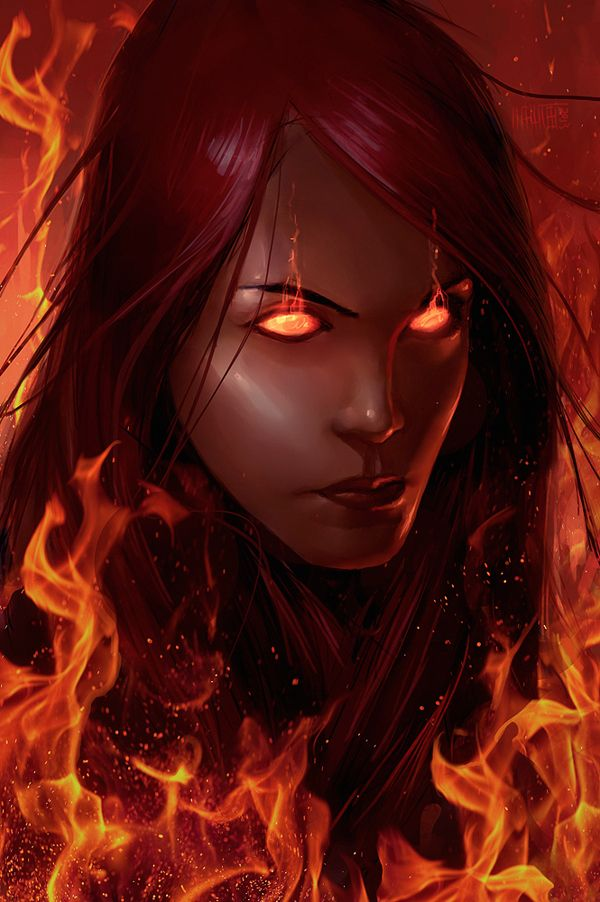
\includegraphics[width=4cm]{images/portrait.png}}
            &
            \begin{tabu}{XX[2]}
                \toprule
                \textbf{Name}                & \textbf{\Large \emph{fubar}}\\
                \textbf{Also known as\ldots} & \\
                \textbf{Personality}         & \\
                \midrule
                \textbf{Gender}              & \\
                \textbf{Height}              & \\
                \textbf{Built}               & \\
                \midrule
                \textbf{Hair}                & \\
                \textbf{Eye}                 & \\
                \textbf{Ethnicity}           & \\
                \midrule
                \textbf{Nature}              & \\
                \textbf{Demeanour}           & \\
                \textbf{Idiosyncrasies}      & \\
                \midrule
                \textbf{Phobia}              & \\
                \textbf{Fears}               & \\
                \textbf{Hopes}               & \\
                \midrule
                \textbf{Summary}             & \\
                \midrule
            \end{tabu} \\
        \end{tabu}
    \end{framed}
    \caption{Character quick summary.}
\label{tab:character-quick-summary}
\end{table*}


\lipsum[1]

\lipsum[2]

\lipsum[3]

\lipsum[4]

\lipsum[5]

\lipsum[6]

\chapter{The story so far\ldots}

\begin{table*}
    \begin{framed}
        \centering
        \taburulecolor |grey!50|{steelblue} \arrayrulewidth=1pt
            \begin{tabu}{X[1]X[2]}
                \toprule
                \textbf{Name} \big[Nicknames\big] & \textbf{ook} \big[\emph{fubar}\big] \\
                \midrule
                Relationship        & \\
                Appearance          & \\
                \midrule
                Nature / Demeanour  & \\
                Idiosyncrasies      & \\
                \midrule
                Summary             & \\
                \bottomrule
        \end{tabu}
    \end{framed}
    \caption{NPC.}
\label{tab:npc-quick-summary}
\end{table*}


\chapter{Character details}

\chapter{Rumours and facts for other players}

% End document
\end{document}
